\documentclass[dvipdfmx]{standalone}
\usepackage{tikz}
\usetikzlibrary{positioning}

\begin{document}
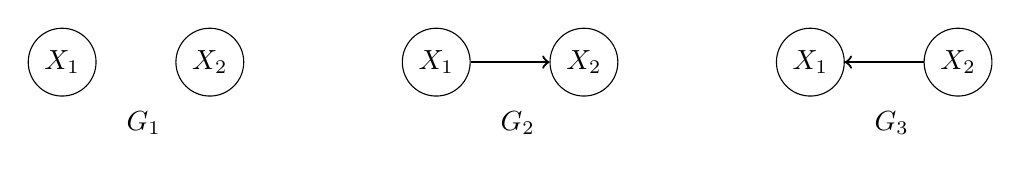
\begin{tikzpicture}[
  nodestyle/.style={
        draw,
        circle
  }
]

    \coordinate (G) at (0cm, 0cm);

    \node[nodestyle] (X1_1) {$X_1$};
    \node[nodestyle, right=1cm of X1_1] (X2_1) {$X_2$}
    node[below left = 0.5cm and 0.5cm of X2_1.center]{$G_1$};
    \node[nodestyle, right=2cm of X2_1] (X1_2) {$X_1$};
    \node[nodestyle, right=1cm of X1_2] (X2_2) {$X_2$}
    node[below left = 0.5cm and 0.5cm of X2_2.center]{$G_2$};
    \node[nodestyle, right=2cm of X2_2] (X1_3) {$X_1$};
    \node[nodestyle, right=1cm of X1_3] (X2_3) {$X_2$}
    node[below left = 0.5cm and 0.5cm of X2_3.center]{$G_3$};

    \draw[thick, ->] (X1_2) -- (X2_2);
    \draw[thick, ->] (X2_3) -- (X1_3);
\end{tikzpicture}
\end{document}
